%! program = pdflatex

%\documentclass[12pt,a4paper]{memoir} % for a long document
%\documentclass[12pt,a4paper,article]{memoir} % for a short document
%\usepackage[pdftex]{graphicx}
%\usepackage{rotating}

% See the ``Memoir customise'' template for some common customisations
% Don't forget to read the Memoir manual: memman.pdf

%\title{NuSim Aspect Reconstruction Verification}
%\author{Kristin Kruse Madsen}

%%% BEGIN DOCUMENT
%\begin{document}

%\maketitle
\chapter{NuSim Aspect Reconstruction Verification Document}
\section{Purpose}
The purpose of this memo is to document the stability and error of the aspect reconstruction algorithm used in NuSim. Details on the mathematics of the algorithm can be found in the NuSim manual. 

The aspect reconstruction algorithm relies on the metrology system and the star tracker to solve for the motion between the Focal Plane Bench and the Optics Bench. Any motion which keeps the planes of the two benches parallel can be fully solved. Tilting of the benches with respect to each other is, however, interpreted as a linear displacement. This causes an error in the solution and it is this error we will quantify here. 

The results shown here were made using NuSim revision 174.

\section{Test description}
In order to probe the stability of the aspect reconstruction several tests were run using five different alignment databases. The databases are all based on the version NuSIM\_OrientationsIDEAL\_007. The databases used were: 

\begin{itemize}
\item NuSIM\_OrientationsDB\_007PL: Purely linear displacement of the benches.
\item NuSIM\_OrientationsDB\_007Rot: Pure tilt of the benches.
\item SAA90DB\_007: Solar Azimuth Angle 90 degree mast bend.
\item SAA135DB\_007: Solar Azimuth Angle 135 degree mast bend.
\item SAA170DB\_007: Solar Azimuth Angle 170 degree mast bend.
\end{itemize}

In revision 174 NuSim has an error when the source is at (Ra,Dec)=(0,0) degrees, therefore tests were run using a point source placed on-axis at (Ra,Dec)=(0.1,0.1) degrees. At this elevation the cosine scaling effect of the azimuth is essentially = 1. The  detectors were shifted linearly so the spot did not fall on one of the detector gaps. 

In the OpticsEngine scattering was turned off and ghostrays turned off, and the perfect optics option were used instead. The perfect optic option modifies the path of the rays such that the on-axis spot hitting the focal plane at exactly the focal length is a perfect spot. This is in reality an unphysical situation since the NuSTAR optics are conic approximations to a Wolter I and perfect focus is not possible, but in order to eliminate any blurring due to the optics we use this setting. The measurement error terms of the metrology and star tracker engines are disabled as well.

\section{Results}
The results from each database run are shown in plots of four. The top panel of the plots shows the residual between the aspect reconstructed source and the actual source input position in arcseconds as a function of time. As explained above we are using a perfect optic, but as will be shown in the linear case the residuals have a 'natural' width. The reason for the width is due to the fact that an event is not deposited at the top of the detector, but typically gets deposited somewhere inside the detector strata. This depth effect causes the spot to diverge, since it was designed to focus at the top of the detector. The natural width of the spot is therefore 0.1 arcseconds.

The two bottom plots show the difference between the location of the optical axis on the sky and the input source position. Whenever there are tilts involved, the optical axis will be offset from the source. These plots trace the amount of tilting in the system.

\subsection{Purely linear displacement}
As stated above, a pure linear displacement of the benches can be exactly solved. This is shown in Figure \ref{test2} which just displays the natural widening of the spot due to the depth effect.

\subsection{Pure tilt of the benches}
The "tilted" database has a rate of 1''/second around the X-axis. Figure \ref{test6} bottom panels shows the tilt of the benches with respect to the celestial coordinates, and had the source been located at exactly Ra,Dec = (0,0) the motion would have been exclusively sensed in Ra. Since the source is at (0.1,0.1) there is a slight mixing of angles, and some of the motion is therefore sensed in the declination.

The top panels show the error due to the tilting. For Ra it can be seen that approximately 100 arcseconds tilt gives rise to a 1 arcsecond error in the aspect reconstruction. As a reference the average angular size of the pixel at this elevation is 12 arcseconds. The declination plot shows the effect of the bench moving away from the focus plane due to the tilt. Away from the plane of focus the spot of the source becomes a doughnut and that is the reason for the branching.

\subsection{Mast bending}
Figure \ref{test3}, \ref{test4} and \ref{test5} show the results of using the mast bending databases. Just as for the situation with a pure tilt, the bottom plots track the magnitude of the tilt, and that tilt is mirrored by roughly a 1/100 residual error in the top plots.

\section{Conclusion}
The residuals of the tilting of the benches is shown to be approximately 1'' per 100'' tilt. In principle the difference between the optical axis and the source can be used to correct the error, however, this requires precise knowledge of the spacecraft bus movement, since any rotation of the entire ridged space craft structure will add to the optical axis path and must be backed out before applying the correction.

The mast database test shows that the residuals even for SAA170, are only 2 arcseconds, which is less than 1/5th of a pixel. 

\begin{figure}[htbp] %  figure placement: here, top, bottom, or page
   \centering
   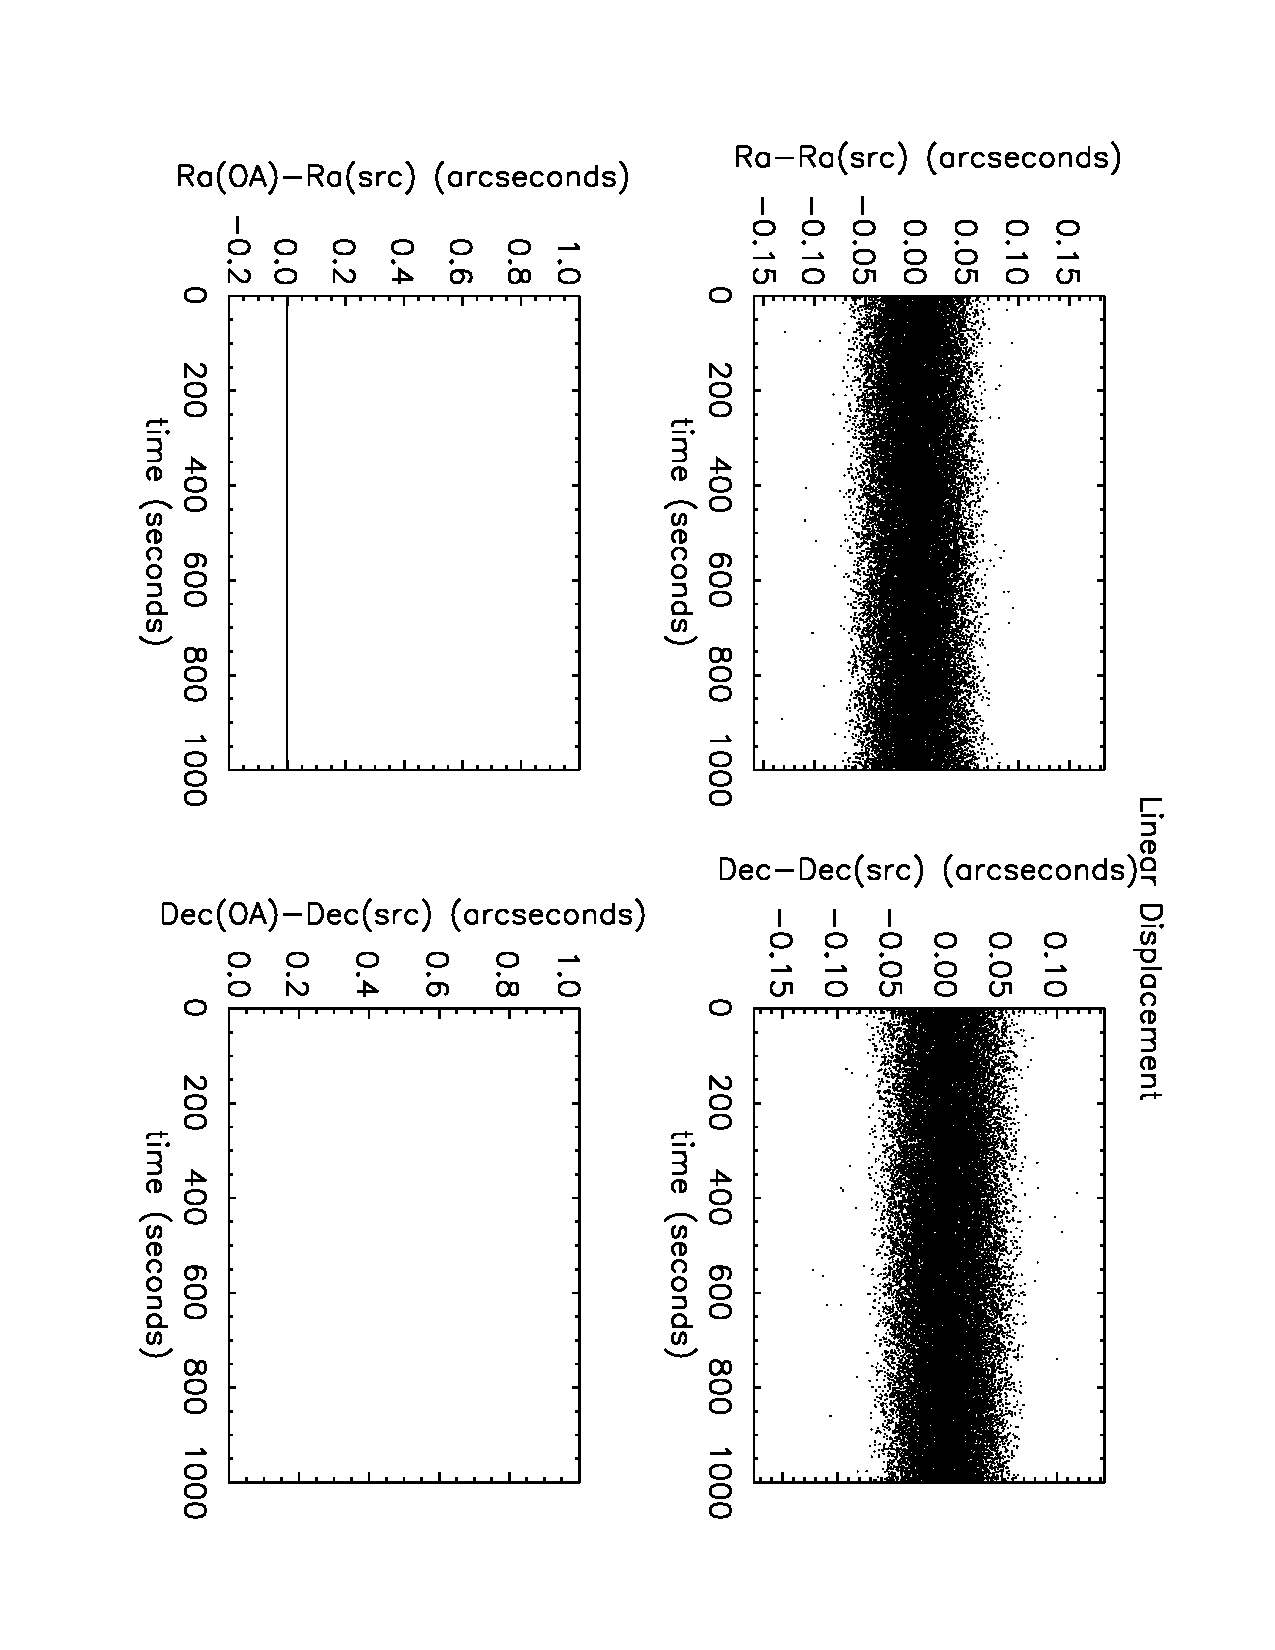
\includegraphics[width=14cm,angle=180]{images/test2.pdf} 
   \caption{\footnotesize{Aspect reconstruction of a linear displacement of the benches. Top panel shows the residual of the reconstruction source position and the actual source position. Bottom panels shows the offset between the source position and the optical axis.}}
   \label{test2}
\end{figure}
\begin{figure}[htbp] %  figure placement: here, top, bottom, or page
   \centering
   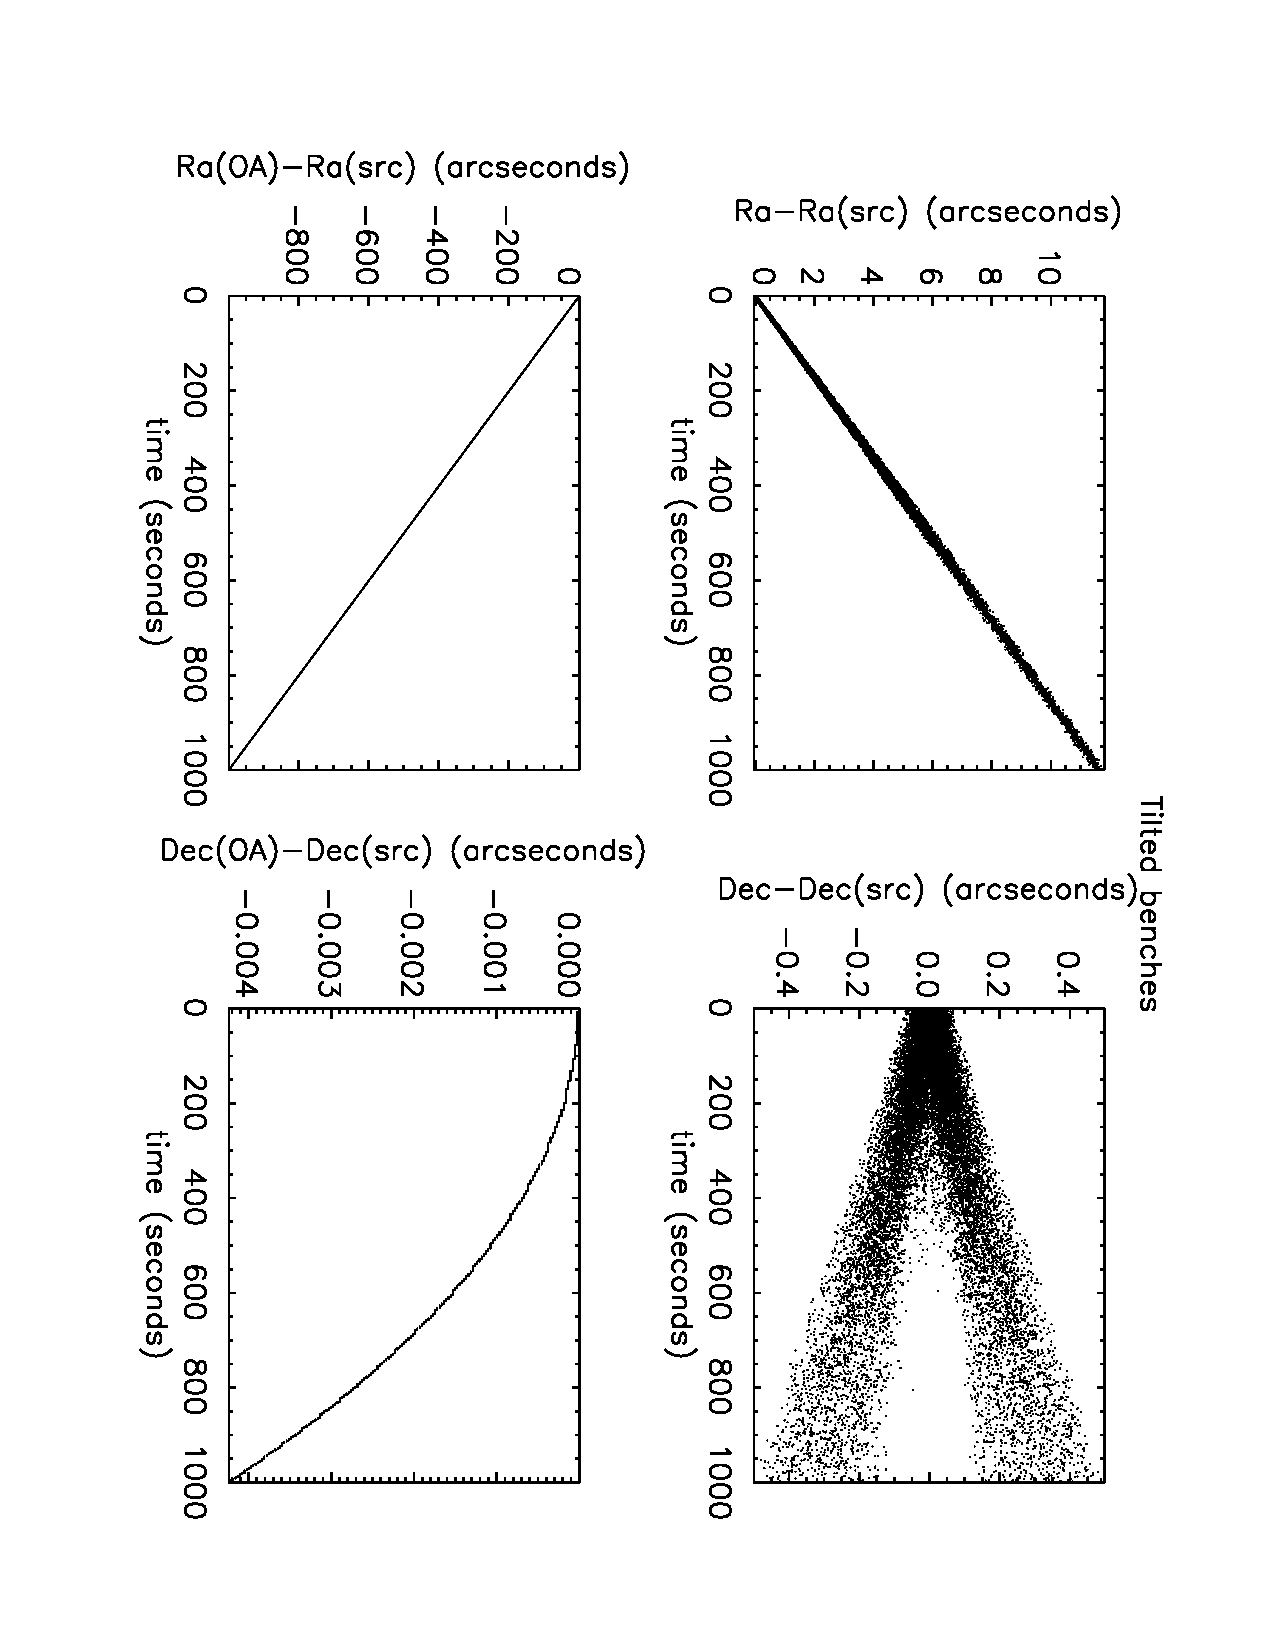
\includegraphics[width=14cm, angle=180]{images/test6.pdf} 
   \caption{\footnotesize{Aspect reconstruction of a pure tilt between the two benches. The rate of tilt is 1''/second. Top panel shows the residual of the reconstruction source position and the actual source position. Bottom panels shows the offset between the source position and the optical axis.}}
   \label{test6}
\end{figure}
\begin{figure}[htbp] %  figure placement: here, top, bottom, or page
   \centering
   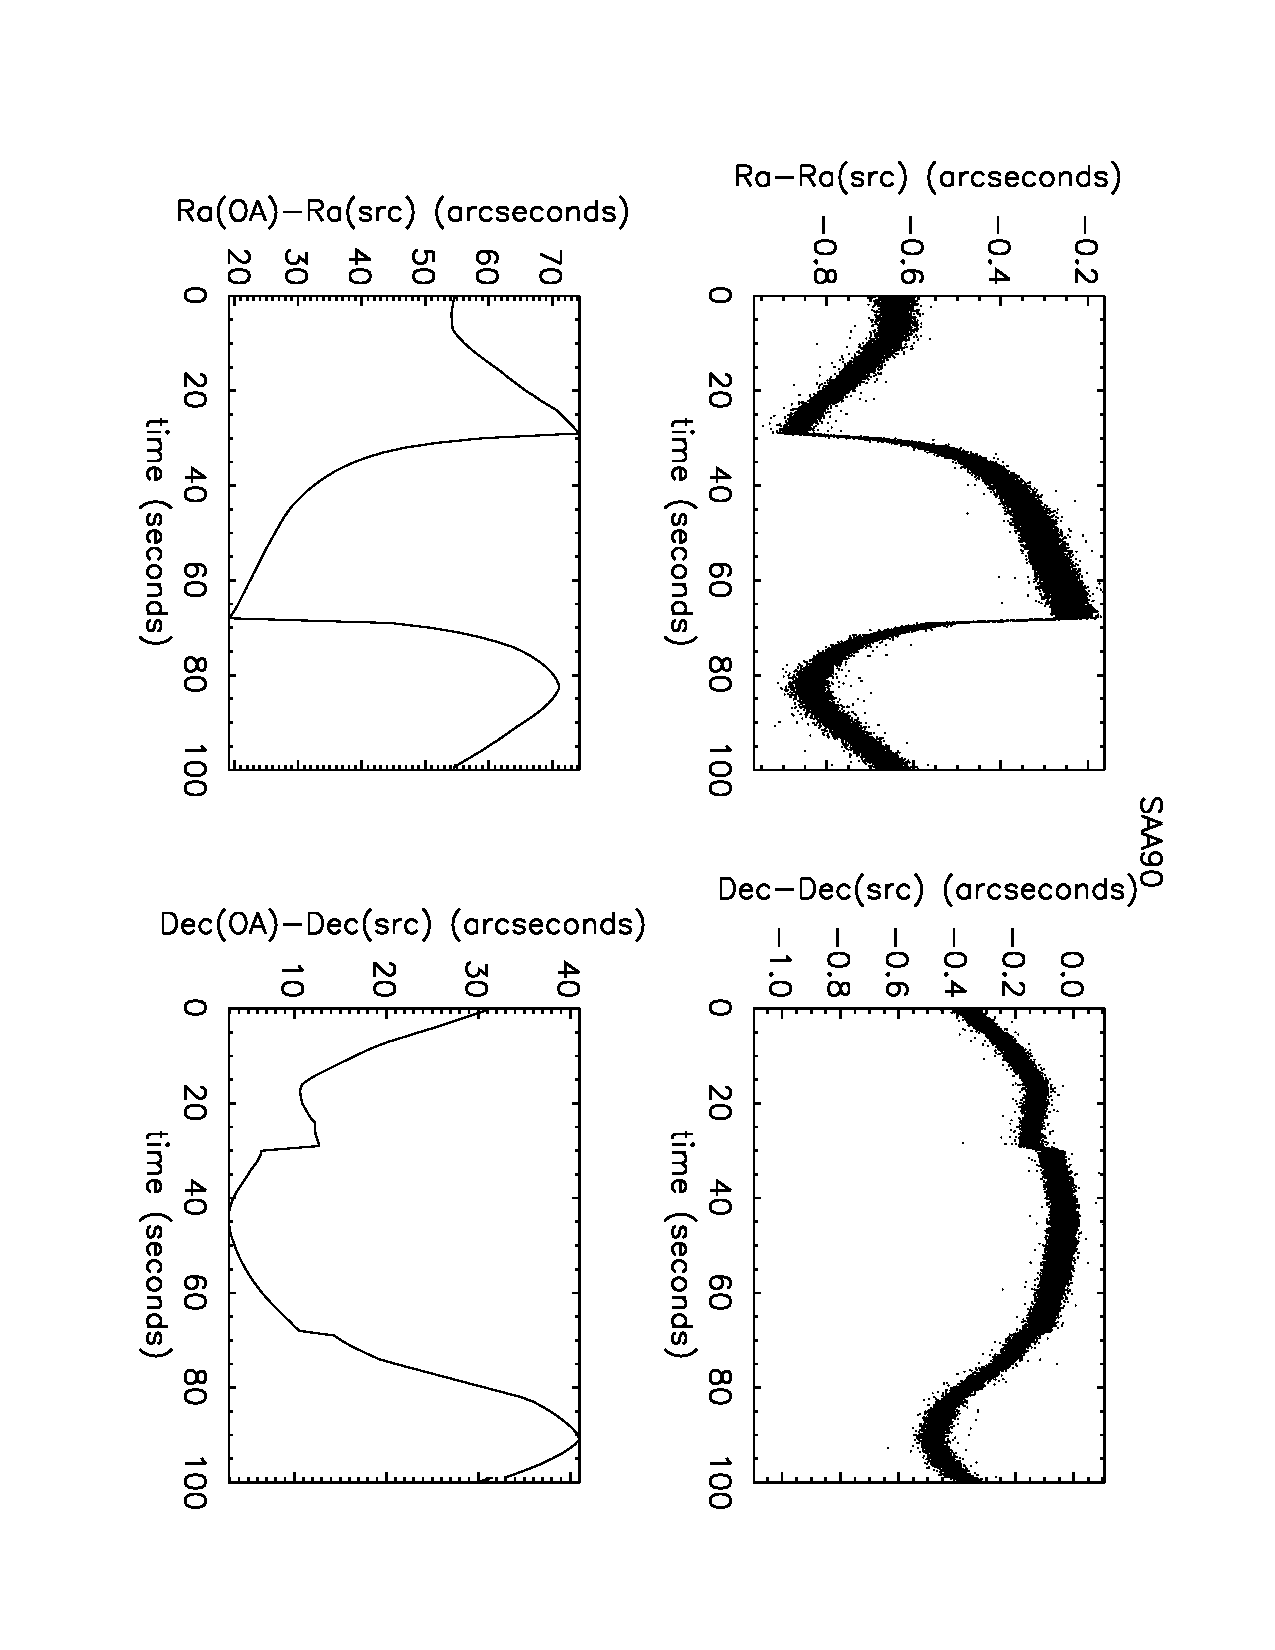
\includegraphics[width=14cm, angle=180]{images/test3.pdf} 
   \caption{\footnotesize{Aspect reconstruction of mast bend database: mastDB90. Top panel shows the residual of the reconstruction source position and the actual source position. Bottom panels shows the offset between the source position and the optical axis.}}
   \label{test3}
\end{figure}
\begin{figure}[htbp] %  figure placement: here, top, bottom, or page
   \centering
   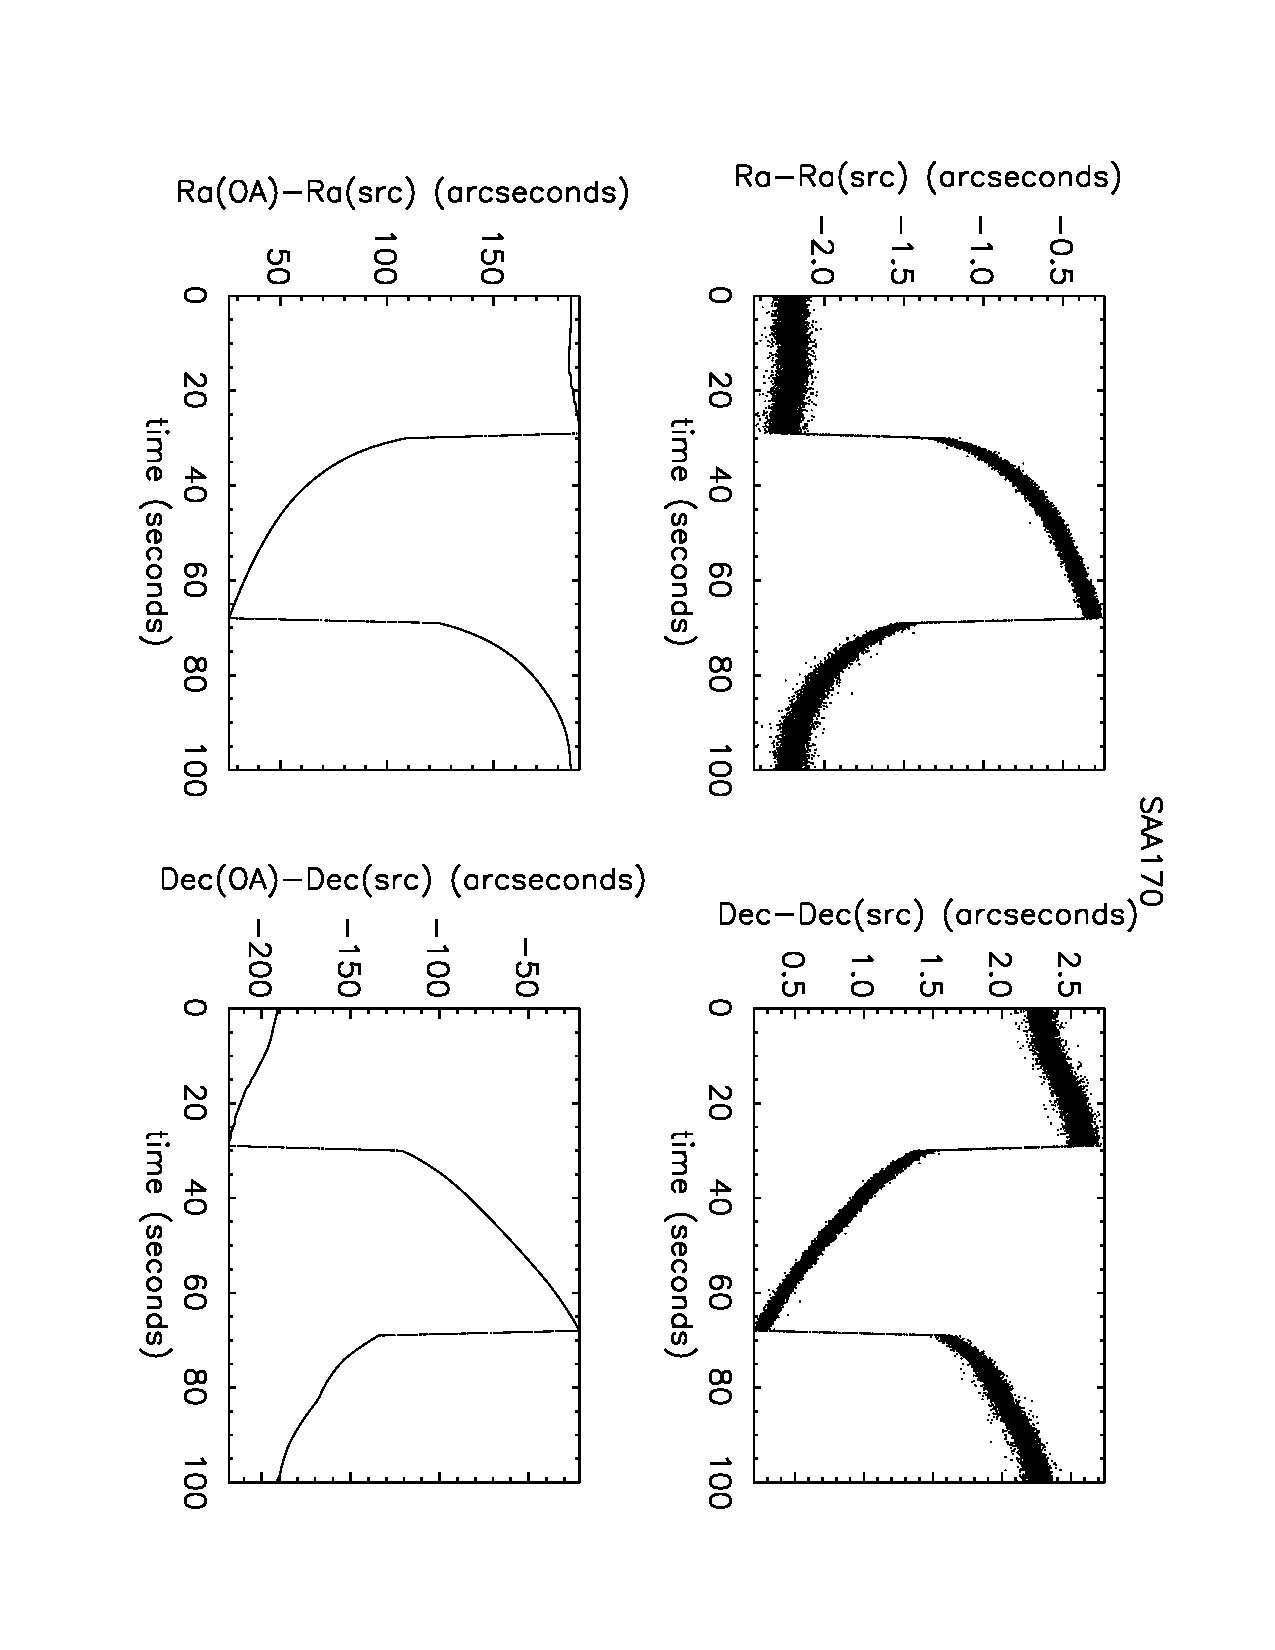
\includegraphics[width=14cm, angle=180]{images/test4.pdf} 
   \caption{\footnotesize{Aspect reconstruction of mast bend database: mastDB170.Top panel shows the residual of the reconstruction source position and the actual source position. Bottom panels shows the offset between the source position and the optical axis.}}
   \label{test4}
\end{figure}
\begin{figure}[htbp] %  figure placement: here, top, bottom, or page
   \centering
   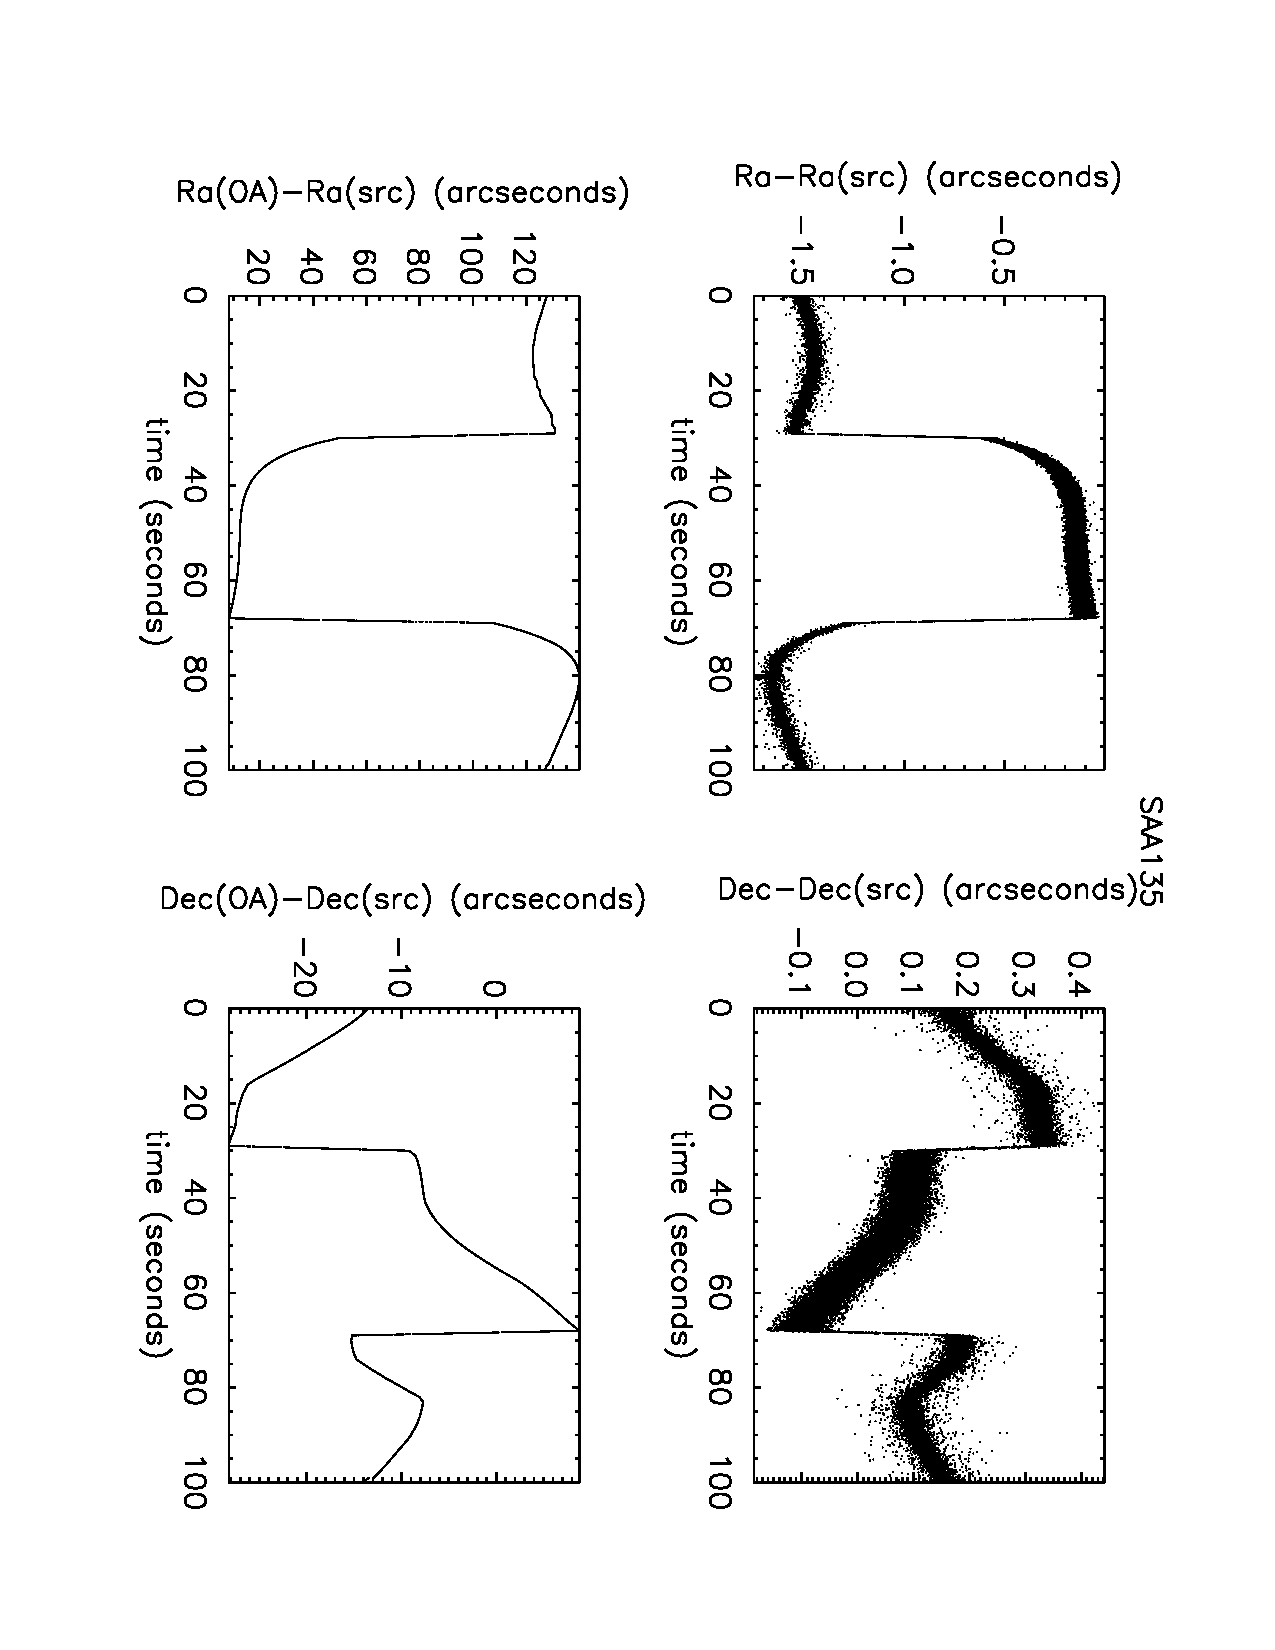
\includegraphics[width=14cm, angle=180]{images/test5.pdf} 
   \caption{\footnotesize{Aspect reconstruction of mast bend database: mastDB90. Top panel shows the residual of the reconstruction source position and the actual source position. Bottom panels shows the offset between the source position and the optical axis.}}
   \label{test5}
\end{figure}


%\end{document}